\documentclass[12pt]{article}
% Load packages
\usepackage{times}
\usepackage{cite}              % Make references as [1-4], not [1,2,3,4]
\usepackage{wrapfig}
\usepackage{simplemargins}
\setleftmargin{1.0in}
\setrightmargin{1.0in}
\settopmargin{1.0in}
\setbottommargin{1.0in}
\usepackage[super]{natbib}
\usepackage{url}                % Formatting web addresses
\usepackage{ifthen}             % Conditional
\usepackage{multicol}                   % Multi-column pages
\usepackage[utf8]{inputenc}     % Unicode support
\usepackage{amsmath}           % Support for writing math formulas
\usepackage{amssymb}           % Support for writing math formulas
\usepackage{epsfig}            % Support separate PostScript files for Fig.s
\usepackage{epstopdf}                   % Converts eps Fig.s to pdf
\usepackage{graphicx}                   % Graphics functions
\usepackage[margin=0.1pt,font=footnotesize,labelfont=bf]{caption}
\usepackage{setspace}                   % Provides line spacing environments
\usepackage{colortbl}
\usepackage[wide]{sidecap}              % Can typeset caption aside the Fig., allows use of margin for Fig.s wider than \textwidth.
\usepackage{supertabular}               % Tables spanning multiple pages
\usepackage{comment}
\usepackage{lineno}
\urlstyle{rm}                                   % URL style
\usepackage{float}
\usepackage[FIGTOPCAP,nooneline]{subfigure}
\captionsetup{font={footnotesize},aboveskip=0pt}        % Styles Fig. captions
%\usepackage[letterpaper,bindingoffset=0.0in,left=1.0in,right=1.0in,top=1.0in,bottom=1.0in,footskip=.25in]{geometry}
\usepackage[font=scriptsize,labelfont=bf]{caption}
\usepackage{blindtext}
\date{}
\usepackage{psfrag}
\usepackage{anyfontsize}
% \doublespacing
\singlespacing
\frenchspacing     % Eliminates double spaces between sentences
\usepackage{titlesec}
\titleformat{\section}
  {\normalfont\bfseries}{\thesection}{1em}{}
\titleformat{\subsection}[runin]
  {\normalfont\itshape}{\thesubsection}{1em}{}
\titleformat{\subsubsection}[runin]
  {\normalfont\itshape}{\thesubsubsection}{1em}{}
\titlespacing*{\section}{0pt}{*1.5}{8pt}
\titlespacing*{\subsection}{0pt}{*1.5}{8pt}
\titlespacing*{\subsubsection}{0pt}{*1.5}{8pt}
\newboolean{publ}
%Publication style settings
%\newenvironment{bmcformat}{\fussy\setboolean{publ}{true}}{\fussy}
\renewcommand{\rmdefault}{ptm}\renewcommand{\sfdefault}{ptm}
\renewcommand{\bibnumfmt}[1]{#1.}    % Change the number format in the ref list
%\renewcommand{\Fig.name}{Fig..}     % Change Fig. to Fig..
%for supplimental material
\newcommand{\beginsupplement}{%
        \setcounter{table}{0}
        \renewcommand{\thetable}{S\arabic{table}}%
        \setcounter{figure}{0}
        \renewcommand{\thefigure}{S\arabic{figure}}%
     }
%%%%%%%%%%%%%%%%%%%%%%%%%%%%%%%%%%%%%%%%%%%%%%%%%%%%%%%%%%%%%%%%%%%%%
%%%%%%%%%%%%%%%%%%%%%%%%%%%%%%%%%%%%%%%%%%%%%%%%%%%%%%%%%%%%%%%%%%%%%
\everymath{\displaystyle}
\begin{document}
%%%%%%%%%%%%%%%%%%%%%%%%%%%%%%%%%%%%%%%%%%%%%%%%%%%%%%%%%%%%%%%%%%%%%
% TITLE PAGE
%%%%%%%%%%%%%%%%%%%%%%%%%%%%%%%%%%%%%%%%%%%%%%%%%%%%%%%%%%%%%%%%%%%%%
\begin{titlepage}
  \begin{center}
    \vspace*{\stretch{0.8}}
    {\LARGE{Towards a Personalized, State Aware Model of Trauma}}\par
    \vspace{5em}
    { \Large{Rachel LeCover} \\
    \vspace{1em}
    { \large{Advisor: Jeffrey D. Varner}}\par   
     \vspace{3em}
    { \large{Qualifying Examination}}\par
     \vspace{1em}
    { \large{August 1, 2016}}\par
    \begin{figure}[h]
    \vspace{3em}
       \centering
       
\includegraphics[width=0.7\textwidth]{figures/CULogo187}
       \end{figure}
    \vspace{2em} \large{ \textit{School of Chemical and Biomolecular Engineering \\ \vspace{0.5em} Cornell University, Ithaca, NY}}}\par
    \vspace{3em}
  \end{center}
\end{titlepage}
\pagebreak
%%%%%%%%%%%%%%%%%%%%%%%%%%%%%%%%%%%%%%%%%%%%%%%%%%%%%%%%%%%%%%%%%%%%%
% INTRODUCTION
%%%%%%%%%%%%%%%%%%%%%%%%%%%%%%%%%%%%%%%%%%%%%%%%%%%%%%%%%%%%%%%%%%%%%
\setcounter{page}{1}
\section*{Abstract}
We propose the development of a personalized, state aware, high fidelity model of traumatic injury. The proposed model will capture both the physical and biochemical aspects of trauma. We have constructed an eight compartment body, with a small wound connected to the arterial compartment. Through a heart rate prediction model, we allowed the volumes of compartments to change based on the concentration of vasoactive factors. Future work will include incorporating more physiological functions into the model as well as personalization.
\section*{Introduction} 
\subsection*{Motivation} 
More than one hundred thousand Americans die of trauma every year, with trauma being the most common cause of death for those under the age of forty-seven, and the third most common for those over that age.\cite{rhee2014increasing} Following deaths caused by the failure of the central nervous system, hemorrhage is the most common cause of death following trauma.\cite{sauaia1995epidemiology,lansink2013cause} Although survival rates for wounded military members have increased since 2005, the same advances have not been made in civilian trauma care, with about 20\% of civilian trauma deaths been deemed preventable. \cite{percentdeaths}

Coagulopathy, a disorder impairing the ability of blood to clot, is one of the three legs of the ``lethal triad", a set of conditions commonly seen in trauma patients. The three legs of the lethal triad feedback on each other, worsening the patient's chance at survival. About a quarter of trauma patients suffer from coagulopathy, and the irreversible bleeding that follows majorly contributes to mortality from trauma. \cite{kauvar2006impact} 
Additionally, patients with coagulopathy but the same Injury Severity Score (ISS) as patients without coagulopathy were more likely to die. \cite{brohi2003acute} Furthermore, the greater the degree of coagulopathy, the higher the mortality rate. \cite{frith2010definition}
For those in the military, hemorrhage is the cause of nearly 90\% of potentially survivable deaths. \cite{blackbourne2010decreasing} This exsanguination can lead to a dilution of coagulation factors in the blood, resulting coagulopathy. In other cases, severe trauma can lead to disseminated intravascular coagulation (DIC), when the balance between coagulation and fibrinalysis shifts and the patient's blood becomes overly prone to clotting. \cite{boccaccio1981disseminated} DIC is a very dangerous condition, with patients suffering from DIC having a much higher mortality rate than other trauma patients. \cite{gando2001disseminated}

At the present, there are no universal guidelines on which fluids an exsanguinating trauma patient should receive. North American hospitals give patients suffering from major hemorrhage fresh frozen plasma, whereas European hospitals would give these patients clotting factor concentrates.\cite{hunt2014bleeding} This is an open area of research, however, it is extremely difficult to perform controlled studies on the efficacy of trauma interventions. Human trauma studies must be performed retrospectively, for ethical reasons. Furthermore, each trauma center has its own procedures, and very few patients have the exact same injury. Therefore, a model of trauma in the human body will allow for potential treatment options to be tested without the need for large scale data collection.

Various trauma associated phenomenon have been modeled at the molecular level: coagulation \cite{luan2007computationally,beltrami1995mathematical,sagar2015dynamic}, fibrinolysis \cite{bannish2012modelling}$^,$\cite{wootton2002experimental}, and compliment\cite{sagar2016reduced,zewde2016quantitative,korotaevskiy2009non}. Several trauma models consider the larger scale physiological effects, but as a rule, these models do not consider the biochemical details.\cite{ho2005mathematical,hirshberg2003minimizing,simpson1996computer,reisner2013computational}  They tend to lump all protein species together (if they are even considered) and contain no information about chemical dynamics. The molecular scale models capture only a piece of trauma, and the large scale models neglect the details of the process. Therefore, there is a need for a model that contains both the physiological information from the whole body models and the biochemical dynamics from the molecular scale models.  
 
\subsection*{Research aims:} The goals of my research are to 
$\boldsymbol{1)}$  Implement a state-aware mathematical model of the human body which captures the biological details of coagulation and fibrinolysis. This model would expand upon already existing differential equation based models of coagulation which use mass action kinetics.
$\boldsymbol{2)}$ Use the model to predict the efficacy of various trauma interventions, such as intravenous fluids.
$\boldsymbol{3)}$ Allow for the personalization of the model based on a subject's physical characteristics.  
%%%%%%%%%%%%%%%%%%%%%%%%%%%%%%%%%%%%%%%%%%%%%%%%%%%%%%%%%%%%%%%%%%%%%
% SIGNIFICANT PREVIOUS WORK
%%%%%%%%%%%%%%%%%%%%%%%%%%%%%%%%%%%%%%%%%%%%%%%%%%%%%%%%%%%%%%%%%%%%%
\section*{Significant Previous Work}
\subsection*{Physiologically Based Pharmoacokinetic Models}
Physiologically based pharmacokentic models, abbreviated as PBPKs, are commonly used to model how substances distribute in living systems, such as the human body. Within the PBPK, the system of interest is divided into several (generally assumed to be well mixed) compartments, with specified flow rates between each compartment and pools of venous and arterial blood, as shown in the simple PBPK in Figure \ref{fig:SamplePBPK}. 
\begin{wrapfigure}{r}{7cm}
        \vspace{-20pt}
        \centering
        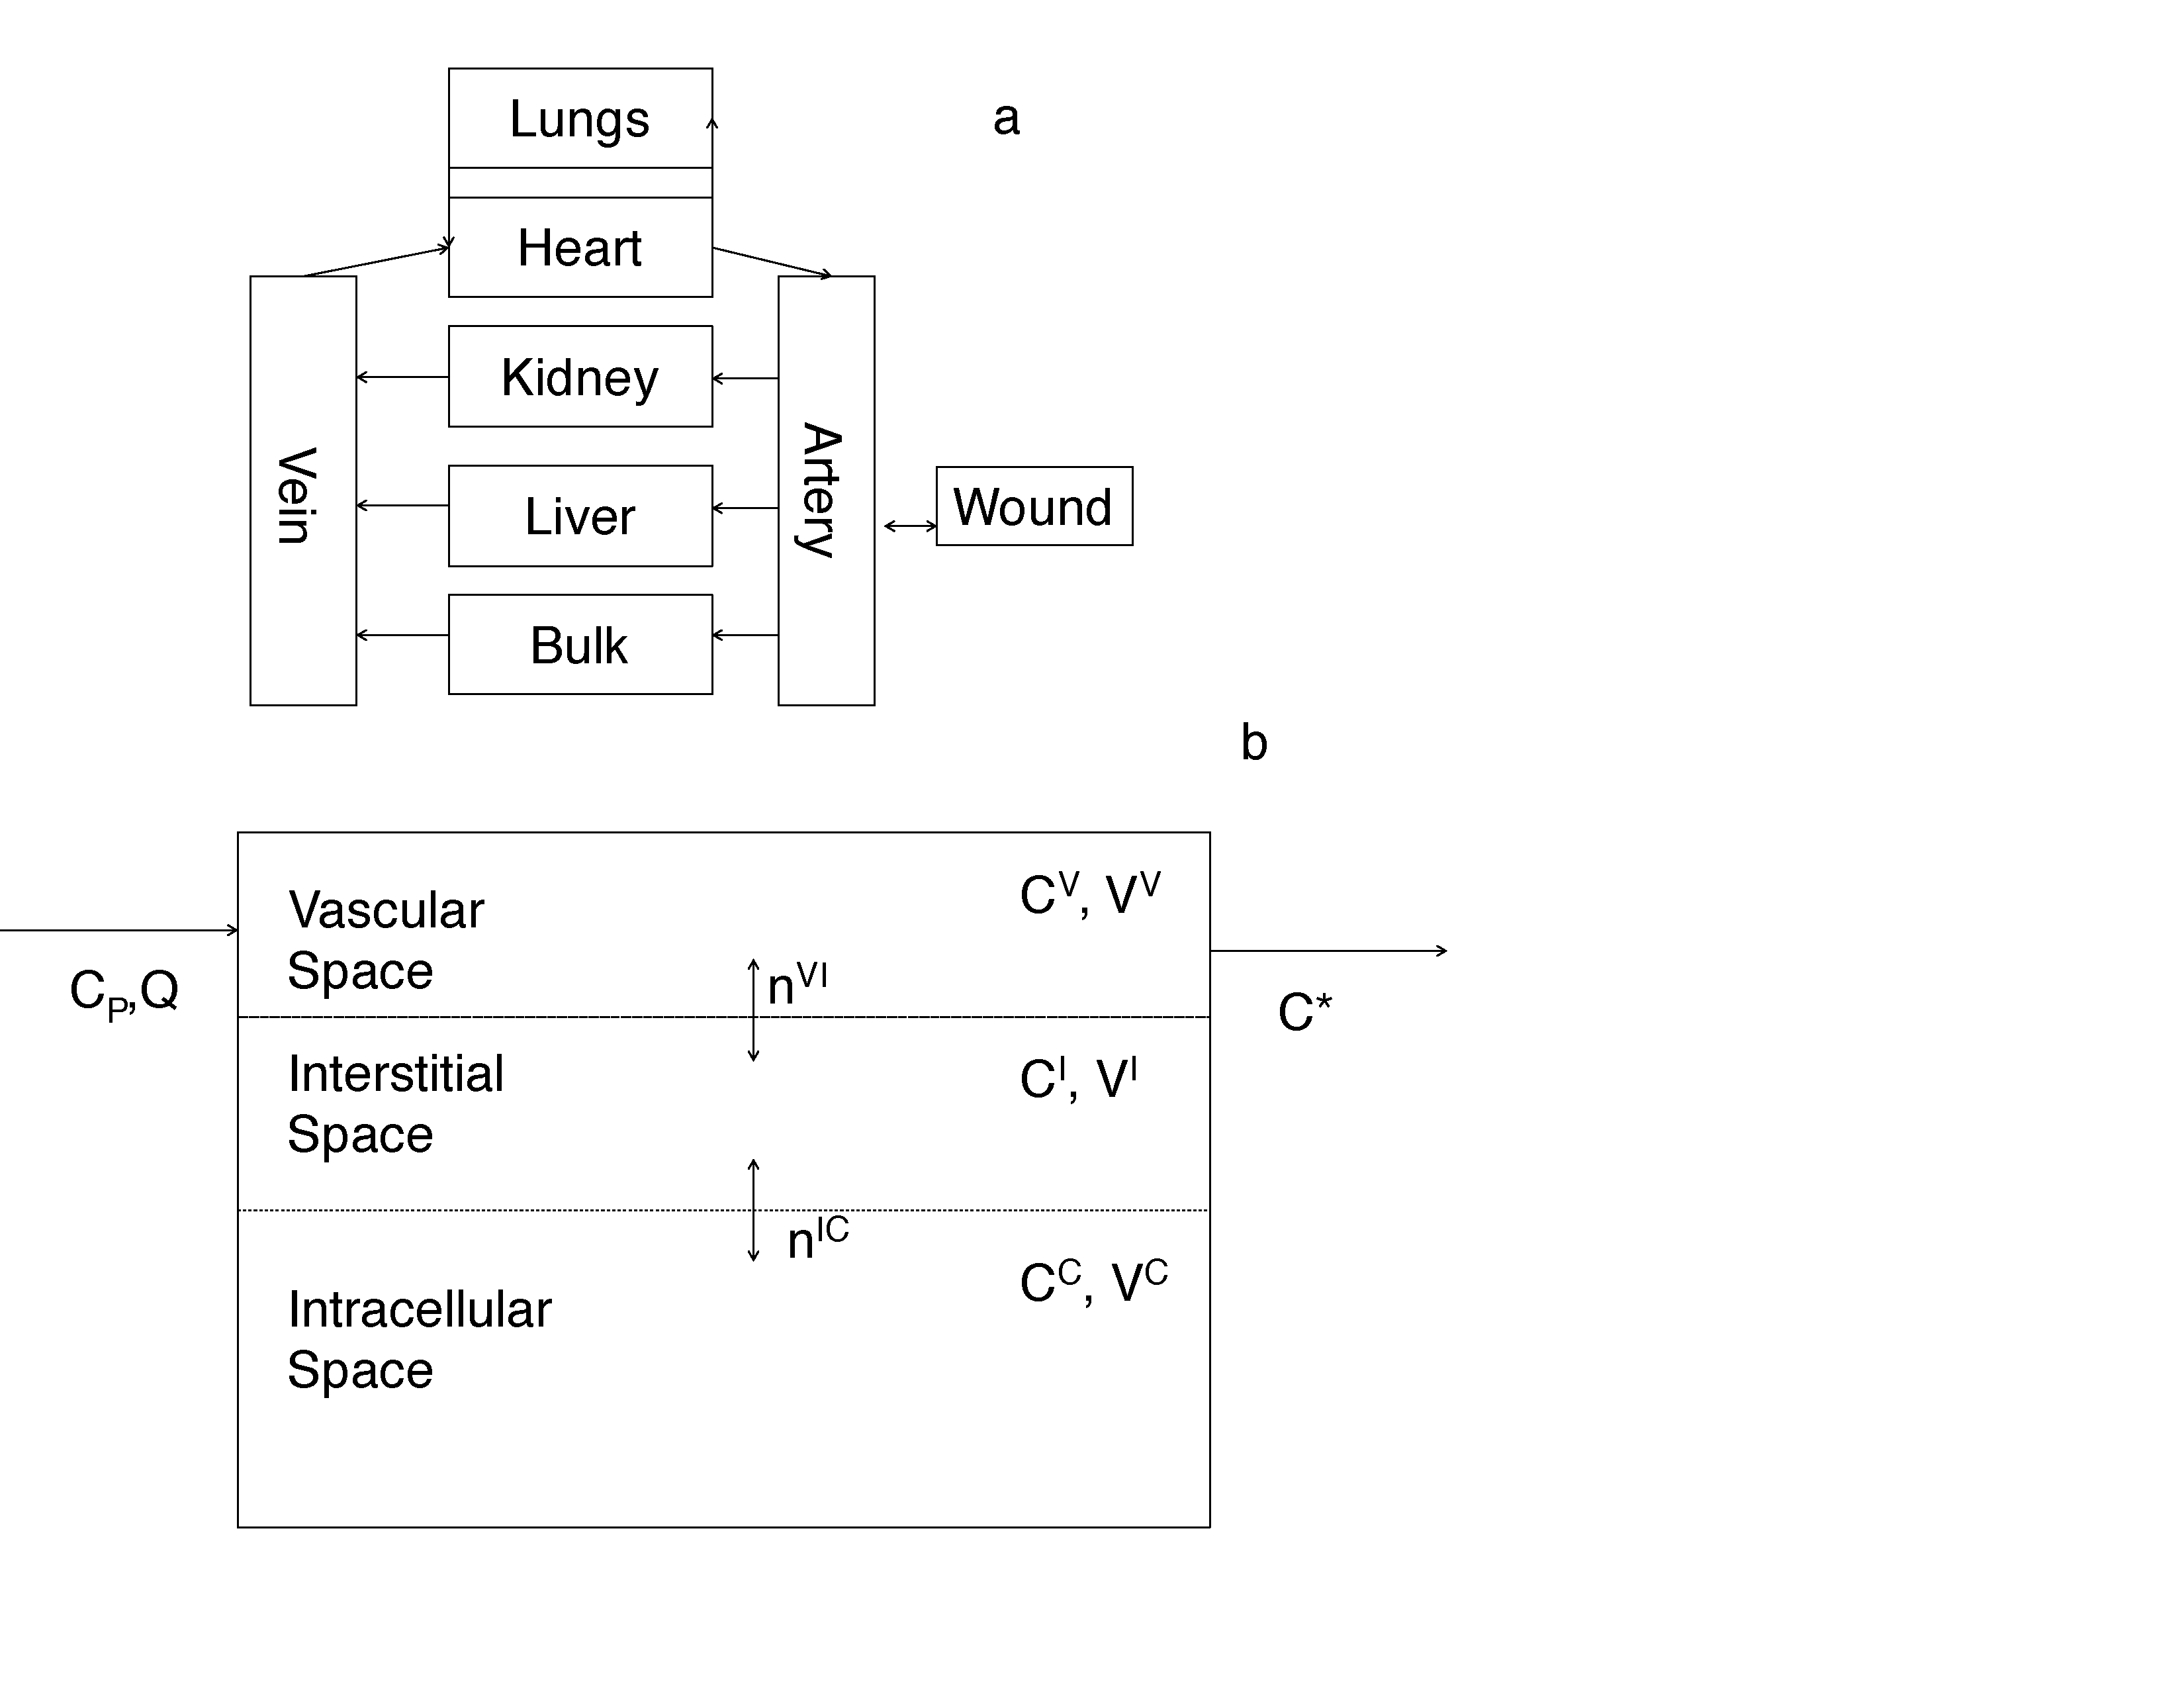
\includegraphics[height=10cm]{figures/bothbodyfigures}
         \vspace{-20pt}
        \caption{\scriptsize Figure a shows a eight compartment PBPK, with arterial and venous blood pools, with a wound off of the aerial blood pool. Figure b shows a sample organ broken up into subcompartments.}
                 \label{fig:SamplePBPK}
\end{wrapfigure}    
We can then write mass balances over each compartment and one over the entire system and solve them to describe the distribution of the substance of interest over time. 
In some cases, each compartment is broken into subcompartments to create a more accurate model, as shown in Figure \ref{fig:SamplePBPK}.
We then write mass balances over the various compartments of the $i^{th}$ organ. 
\begin{equation}
V^V_i\frac{dC^V_i}{dt} = Q_iC_p-Q_iC_i^V-n_i^{V-I}
\end{equation}
\begin{equation}
V^I_i\frac{dC^I_i}{dt} =n_i^{V-I}-n_i^{V-C}
\end{equation}
\begin{equation}
V^C_i\frac{dC^C_i}{dt} =n_i^{I-C}
\end{equation}
The superscript V denotes vascular, I interstitial, P plasma, and C cellular, $n_i$ describes the flux between compartments, $Q_i$ gives the flow rate between compartments, and $C_i$ is the concentration in the $i^{th}$ compartment. \citep{clewell2007physiologically} The volumes of the compartments are assumed to be constant, so dilution terms are neglected. We can use the PBPK technique of modeling the body as different compartments as a frame for our trauma model.
\subsection*{Coagulation and Fibrinolysis}
Historically, the coagulation cascade was considered to be two distinct pathways, the extrinsic and intrinsic, but today, it is known that the two pathways are linked.\cite{adams2009review} 
\subsubsection*{Clot Formation}
The coagulation process begins when an injury occurs, which exposes tissue factor, a transmembrane protein expressed on the surface of cells surrounding blood vessels. \citep{mackman2009role} The newly exposed tissue factor can then bind to factor VIIa (FVIIa), thus forming the extrinsic tenase complex. Then, the extrinsic tenase complex catalyzes the conversion of FX and FIX to their active forms, FXa and FIXa. \cite{mann2006models} FXa converts a small amount of prothrombin to thrombin, and this thrombin then activates FV, FVIII, and FXIII giving rise to FVa, FVIIIa, FXIIIa.\cite{orfeo2004factor} Thrombin also binds to G-coupled protein receptors on platelet membranes, activating the platelets and inducing them to aggregate.\citep{hoffman2009hematology} FIXa and FVIIIa form the intrinsic factor tenase complex, which strongly converts FX to FXa, leading to a large increase in thrombin production. FXa and FVa bind together to form the prothrombinase complex, which converts prothrombin to thrombin about $10^8$ times efficiently as FXa alone. \cite{walker1994activation} The large amount of thrombin produced leads to the conversion of fibrinogen to fibrin, and FXIIIa helps cross link the fibrin to form a stable network, leading to the formation of a clot. \cite{hoffman2009hematology}
%Coagulation has been modelled at varying levels of detail. This process has been modelled in great detail using ordinary differential equations, keeping track of 92 proteins and 148 protein-protein interactions, with each reaction modelled using mass action kinetics. \cite{luan2007computationally}  Additionally, it has been modeled as a set of positive feedback loops, with the last loop further activating the first loop.\cite{beltrami1995mathematical} More recently, Varner et al created a reduced order model of coagulation by combining ordinary differential equations with logical rules. \cite{sagar2015dynamic} This reduced order model contains only five differential equations, making it much less computationally intensive to solve. 
\subsubsection*{Clotting Regulation}
The clot formation process, with respect to thrombin, is a positive feedback loop with a small amount of thrombin leading to the generation of large amounts. This process can be stopped by several different inhibitors, including one activated thrombin: thrombomodulin. Thrombomodulin inhibits the formation of additional thrombin by binding to thrombin (preventing thrombin from activating any other factors), and the thrombin-thrombomodulin complex activates Protein C. \cite{esmon1989roles} Protein C, with its cofactor protein S, inactivates factors Va and VIIIa. \citep{esmon1987anticoagulation}
Tissue factor pathway inhibitor stops the clotting process in two ways: it binds to the FVIIa:TF complex, making it unavailable to produce FXa and FIXa, and it binds to already produced FXa, rendering it inactive. \cite{lwaleed2006tissue} Antithrombin binds to active factors, preventing them from further catalyzing the clotting process. \cite{olson1994regulation}  Protein Z complexes with protein Z-dependent protease inhibitor in plasma, and reduces the activity of FXa, FXIa, and FIXa. \citep {corral2007protein}
Thrombin activated fibrinolysis inhibitor (TAFI) is activated the thrombomodulin-thrombin complex. \citep{chapin2015fibrinolysis}. It removes the lysine and arginine residues form the C-terminal of fibrin, which reduces the number of sites at which plasmiogen can bind, stabilizing the clot. 
\subsection*{Fibrinolysis}
Fibrinolysis, the process that breaks down clots, must be in balance with coagulation, otherwise, coagulopathy or disseminated intravascular coagulation may occur. Plasmin, the enzyme that breaks down clots, has two activators, tPA and uPA. \cite{wiman1978molecular} Tissue plasminogen activator (tPA) or urokinase (uPA) convert plasminogen, the plasmin precursor, to plasmin on the surface of the clot or on cell membranes. \citep{chapin2015fibrinolysis} Both tPA and uPA are serine proteases and have short half-lives in circulation, on the order of 4-8 minutes, before they are destroyed in the liver. Their locations of manufacture differ: tPA is produced endothelial cells, uPA is produced by monocytes and macrophages. Both are inhibited by plasminogen activator inhibitor-1 (PAI-1), and tPA increases dramatically in activity when it binds fibrin. \citep{chapin2015fibrinolysis}
\subsection*{Complement}
Complement, named for its ability to improve the activity of the immune system, also interacts with the coagulation cascade. Complement can be activated by three major pathways: the classical pathway, the lectin pathway, or the alternative pathway. \citep{oikonomopoulou2012interactions} Antigen-antibody complexes trigger the classical pathway, the carbohydrates on the surfaces of microbes initiate the the lectin pathway, and the binding of C3b to properdin or the the spontaneous activation of complement component 3 (C3) by hydrolysis triggers the alternative pathway. All of these pathways intersect with C3 convertase. \citep{markiewski2007complement} 
C3a activates platelets, increasing their tendency to aggregate. C3b is converted into C5 by C3 convertase, resulting in the formation of C5a and C5b. The presence of C5a increases the tendancy of blood to clot by upregulating the production of tissue factor. Although thrombin isn't traditionally included in the compliment pathway, it also plays a role. Thrombin can act on both C3 and C5 to produce C3a,C3b,C5a and C5b, amplifying compliment. \citep{oikonomopoulou2012interactions}
%Bannish created a very detailed model of fibrinolysis using a stochastic model to model tPA binding and combined that with a macrosccale model to measure how fast the lysis front moves. \cite{bannish2012modelling} The dissolution of clots has also been modeled using the Naiver Stokes equation for flow over and through the clots combined with mass balances over the relevant species.\cite{wootton2002experimental} 
%\subsection*{Previous Trauma Models}
%Several whole body models of trauma exist, however, they tend to either simplify the body or the coagulation process. 
%Ho et al developed a model that considered blood to be two distinct parts, either hematocrit or plasma, and assumed that the rate of fluid loss was the same as the rate as fluid replacement. They did not model any of the dynamics of the coagulation process, rather, they lumped all of the coagulation factors into one variable, which they correlated with prothrombin time. \cite{ho2005mathematical} Their model provides guidance on the ratio of fresh frozen plasma (FFP) to packed red blood cells (PRBC) that patients with excessive blood loss should receive. 
%A slightly more complex model by Hirshberg et al modelled blood as having three compartments: red cells, plasma, and water, and allowed flow between these compartments based on systolic blood pressure. \cite{hirshberg2003minimizing} They used prothrombin time to quantify if a patient was at risk for dilutional coagulopathy, and did not consider the biological mechanisms behind coagulation. A model without compartments, but containing more physiological functions was developed by Simpson et al.\cite{simpson1996computer} 
%Simpson's model allows for both blood pressure and bleed out rate to change over time, with the bleed out rate decreasing as blood pressure decreases. This model predicts hematocrit levels over time, but not the levels of specific proteins. 
%Reisner et al re-purposed their model of the cardiovascular system (which was originally created to predict how the cardiovascular system responds to orthostatic stress) to study hemodynamic responses to haemorrhage.\cite{reisner2013computational} Their model includes the heart and pulmonary circulation as well as four peripheral tissue compartments representing the upper body, legs, viscera and kidneys, each of which received the same fraction of the cardiac output. They modelled blood by separating it into two components: red blood cells and plasma. This model includes transcapillary fluid exchange and lymphatic flow, but groups all proteins together. 
%%%%%%%%%%%%%%%%%%%%%%%%%%%%%%%%%%%%%%%%%%%%%%%%%%%%%%%%%%%%%%%%%%%%%
% PRELIMINARY RESULTS
%%%%%%%%%%%%%%%%%%%%%%%%%%%%%%%%%%%%%%%%%%%%%%%%%%%%%%%%%%%%%%%%%%%%%
\section*{Preliminary Results}
\subsection*{Incorporating Reduced Order Model into PBPK}
We constructed an eight compartment model of the human body, using the Kwatee code generation system. In this model, blood flowed from a venous pool, to the heart, through the lungs, back through the heart, an into an arterial blood pool. Blood then passed from the arteries through the liver, kidney, or bulk to the veins. All of the proteins flowed freely between compartments, except for thrombomodulin and trigger, which are bound to cell membranes.\cite{esmon1989roles} We simulated a small wound connected to the arterial blood pool, with a volume of .5\% of the total blood volume, as shown in Figure \ref{fig:SamplePBPK}a.

 We modeled the dynamics of coagulation in each compartment using the reduced order model constructed by Sagar et al.\cite{sagar2015dynamic} In the reduced order model, trigger (which biologically corresponds to to the tissue factor-FVIIa complex) activated thrombin. Thrombin then catalyzed its own activation, as well as the activation of Protein C,which inhibited the activation of thrombin. Antithrombin complexed with thrombin and deactivated it. We ran the model in one hundred different patients, each with slightly different organ volumes and initial concentrations, as shown in Figure \ref{fig:demoPBPK}. The patient is bleeding out at a constant rate of 10.5 mL/min, which would lead to complete exsanguination in a bit less than ten hours. As blood volume diminishes, the heart rate of the patient increases. The blood loss comes from the arterial and bulk compartments, leading to a rise in the concentration in thrombomodulin in those compartments, as their volume is decreasing while the amount of thrombomodulin present remains constant.
\begin{figure}
%\begin{wrapfigure}{R}{\textwidth}
        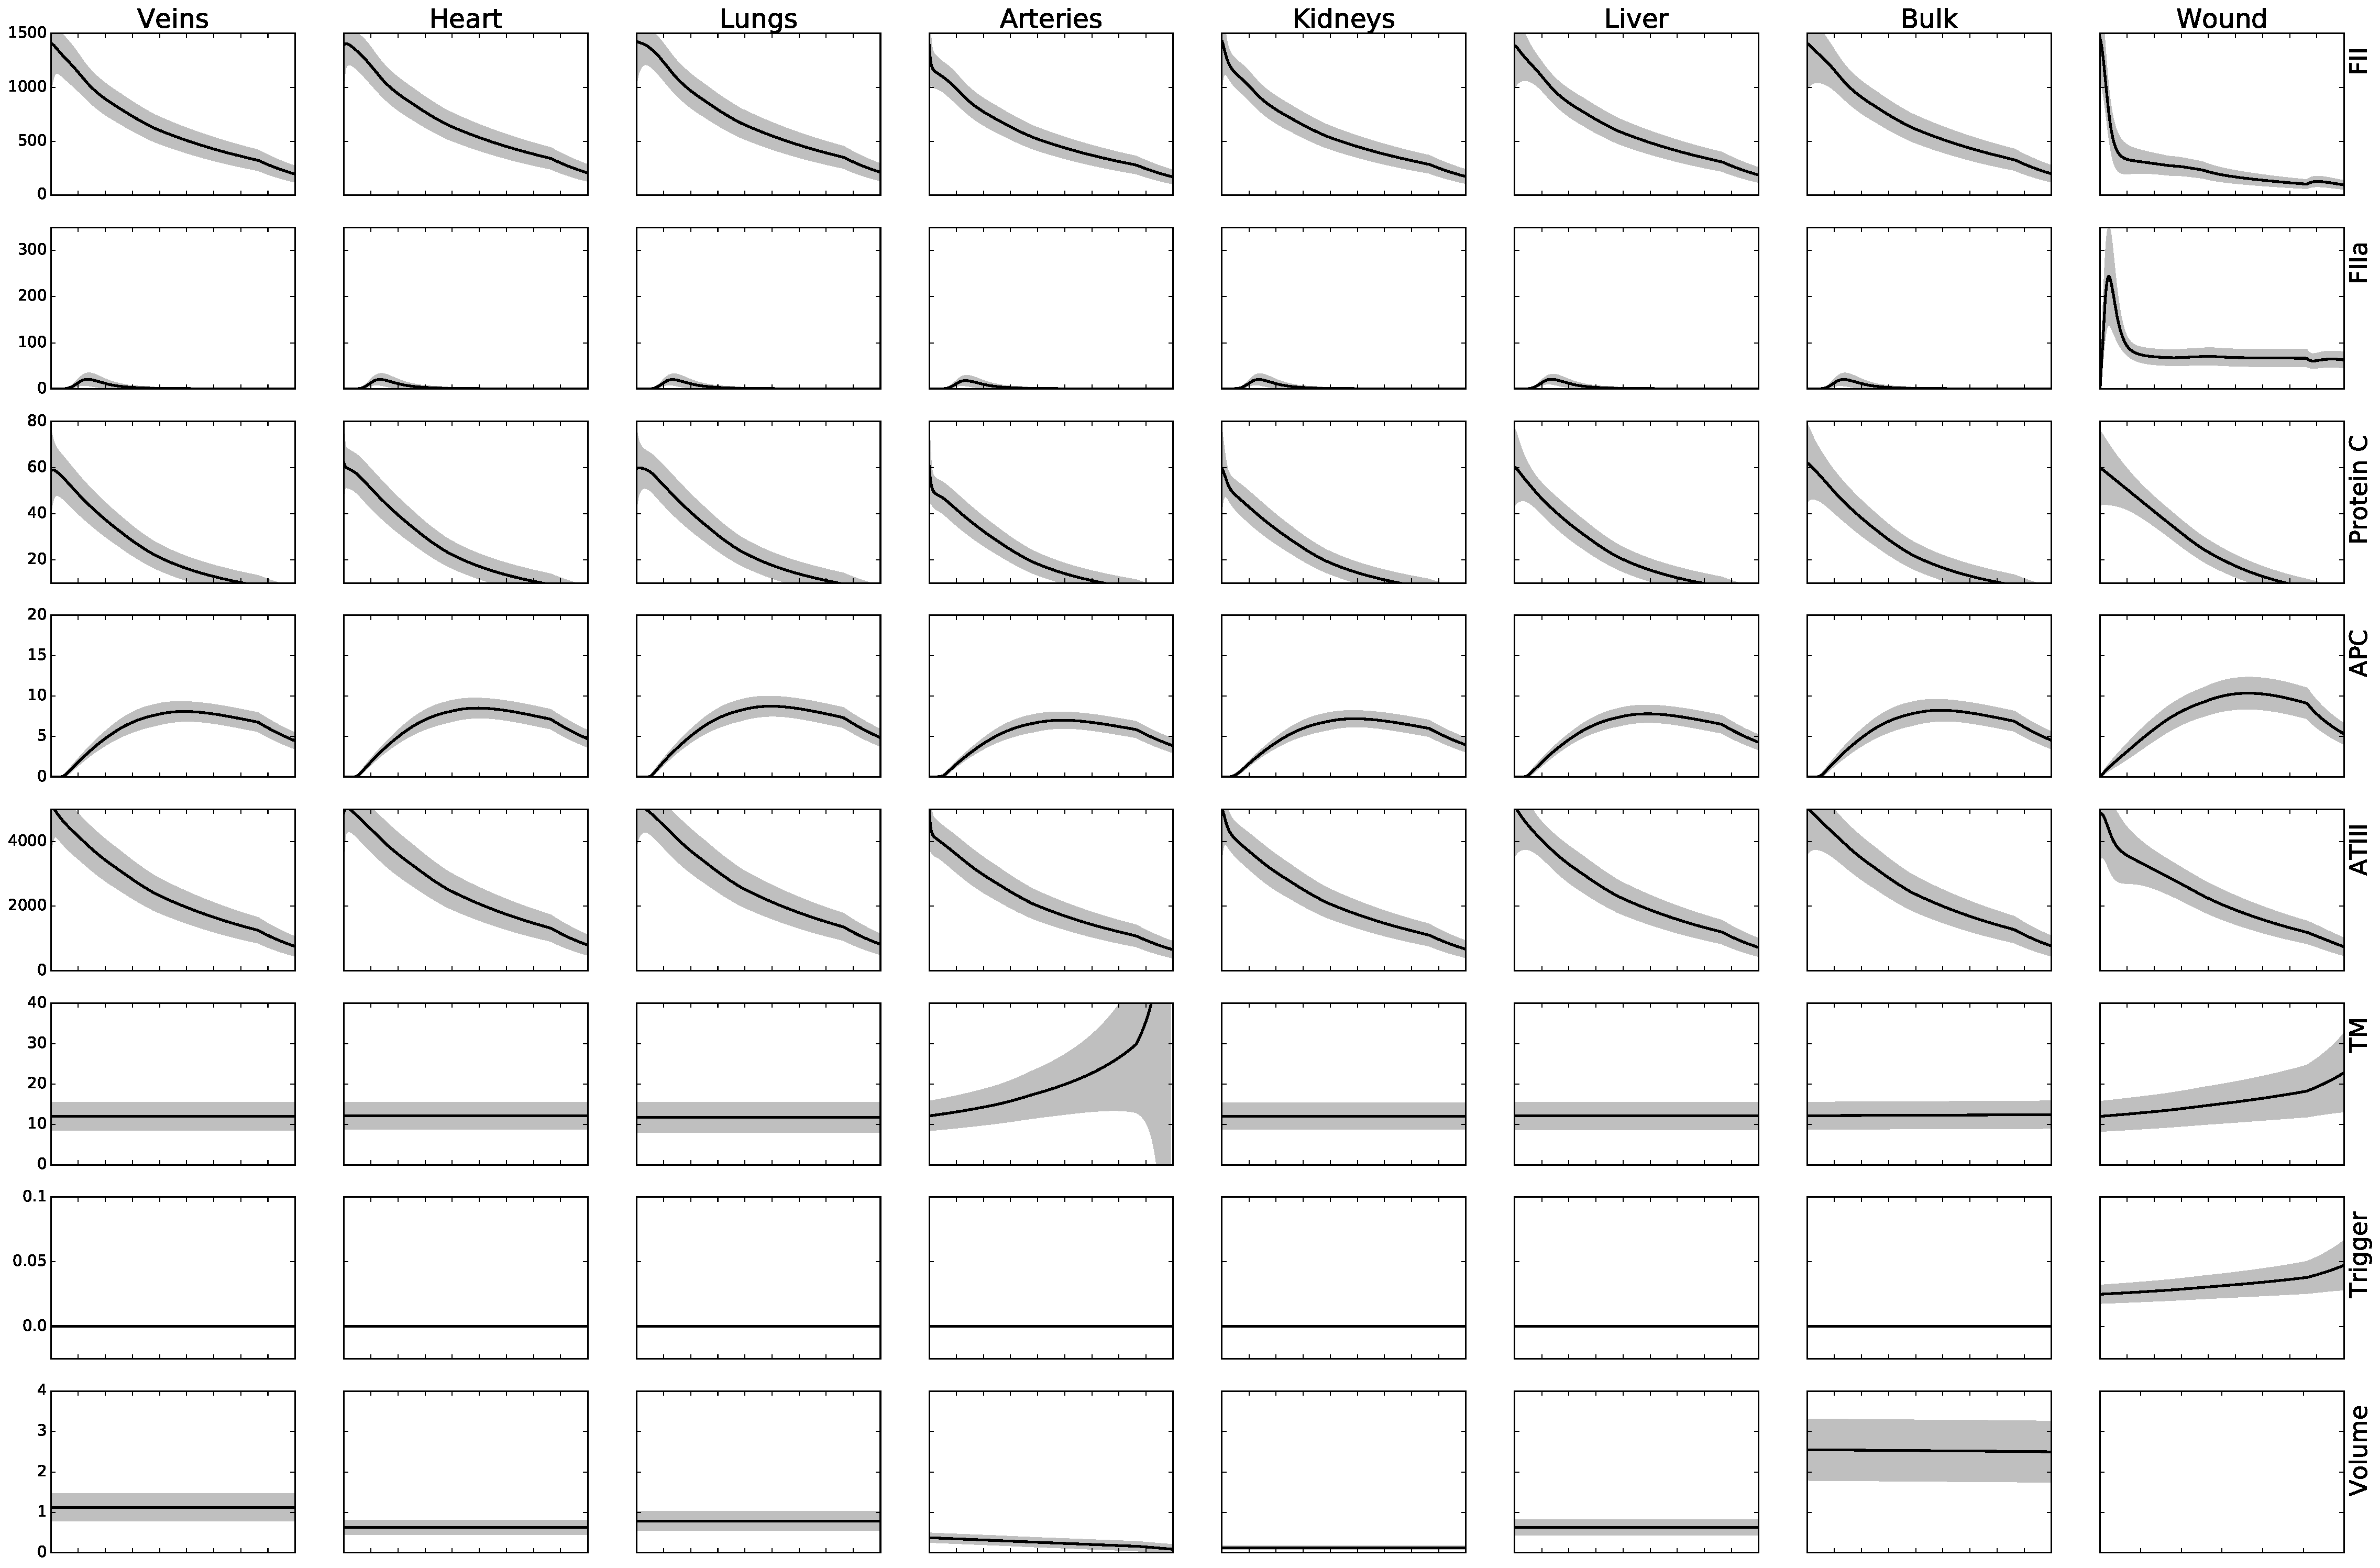
\includegraphics[width=\textwidth]{figures/DifferingInitialVolumesAndConditionsPrettyDiffContraction}
        \caption{\scriptsize All concentrations given in nanomolar, and times in minutes. Each tick on the x-axis represents five minutes. Volumes are given in liters. The black line represents the average response over 100 patients whose initial concentrations were permitted to vary by up to 25\%, as were their organ volumes. The black line is the average response, and the grey is a 95\% confidence interval.}
        \label{fig:demoPBPK}
%\end{wrapfigure}
\end{figure}
\subsection*{PBPK With Changing Heart Rate and Volume Changes}
  \begin{wrapfigure}[40]{r}{.33\textwidth}
        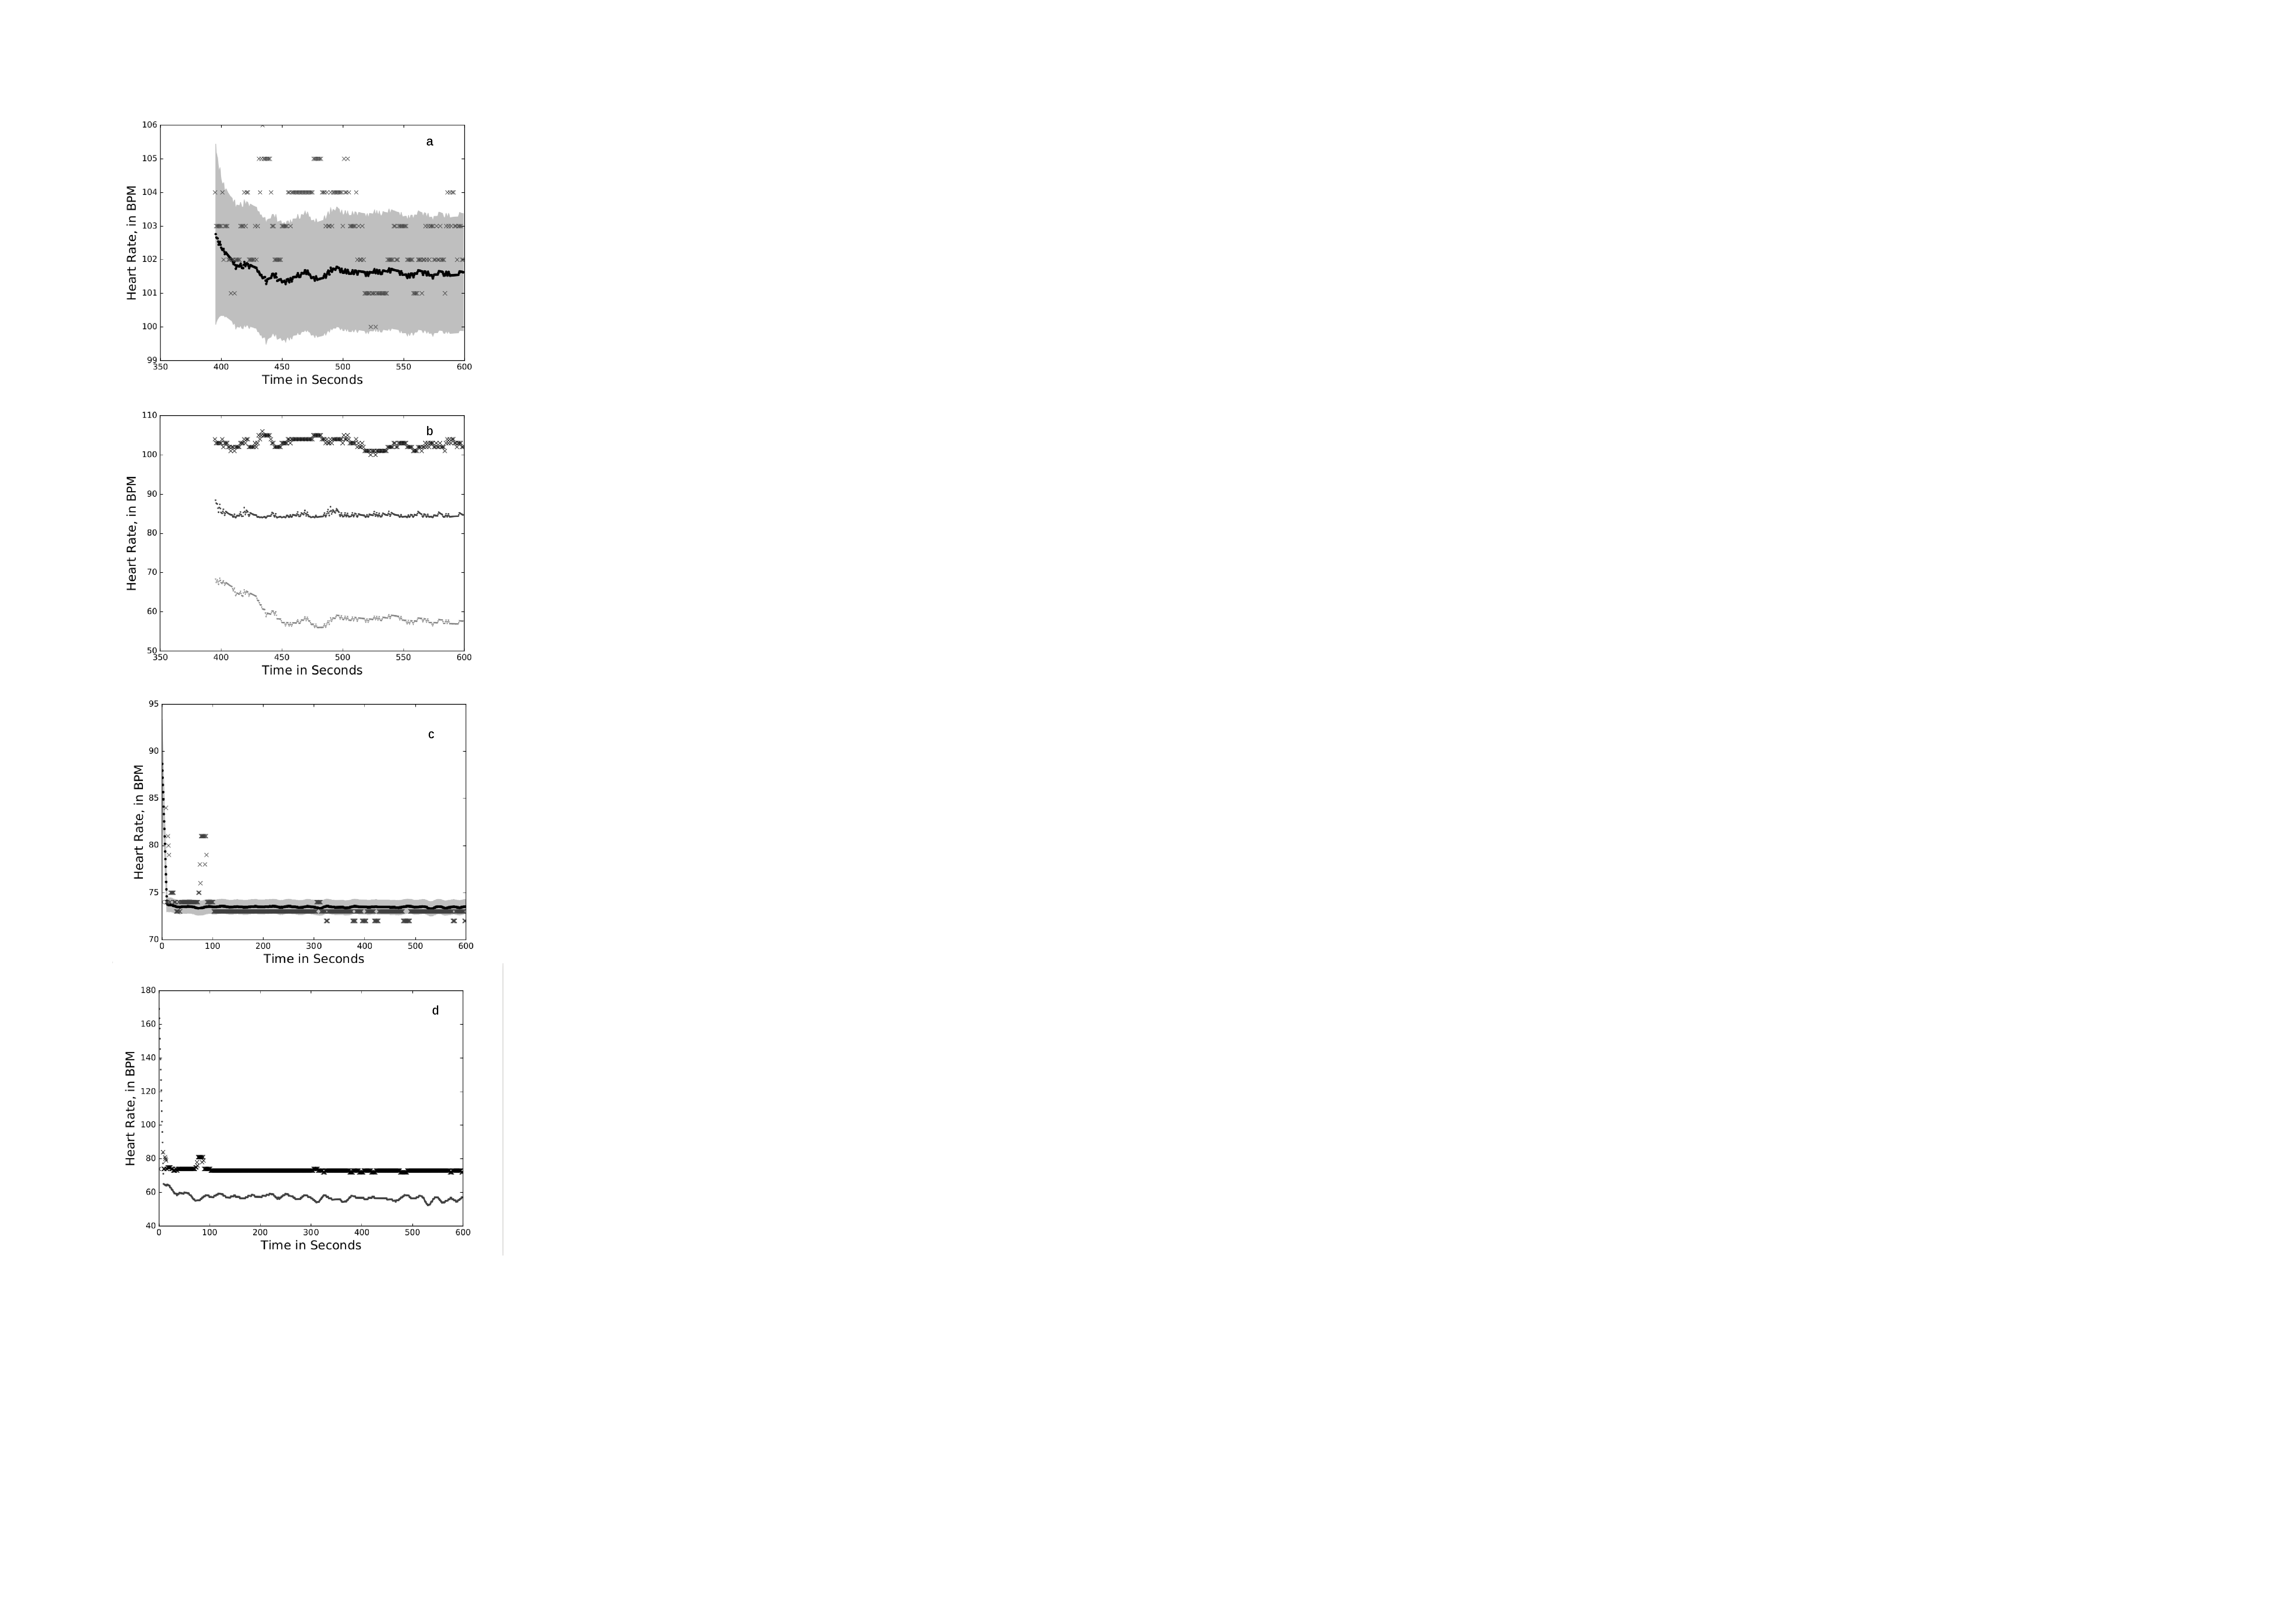
\includegraphics[width=.325\textwidth,trim = {6cm 17cm 94cm 5cm},clip]{figures/OOmodelincol}     
       \caption{\scriptsize The x represent the true data, the black dots represent the average model performance over the 10 different parameter sets, and the grey is a 95\% confidence interval. Figures a and b are cluster 1 patient, Figures c and d show cluster a 2 patient. Subfigures a and c used the parameters estimated by simulated annealing, subfigures b and c show performance of the original parameters in light grey and the parameters estimated by Nelder-Mead in dark grey.}   
       \label{fig:mulitobjperformance}
\end{wrapfigure}
When less than 10\% of blood volume has been lost, the barroreflex kicks in as pressure has dropped to increase heart rate. \cite{foex1999systemic} After approximately 10\% of blood volume has been lost, heart rate begins to decrease, as does blood pressure. When blood loss approaches 30\% of blood volume, heart rate increases dramatically.\cite{jacobsen1990cardiovascular} During all three phases, the concentrations of adrenaline, noradrenaline, and vasopressin rise, but then decrease once blood is transfused.
Using the blood pressure tracks from the MIMIC II numerics data base, we used Olufsen's and Ottsen's model to predict heart rate, and used the predicted heart rate within the PBPK model. \cite{olufsen2013practical} The details of the heart rate prediction model are given in the supplemental material.
 We used the Nelder Mead algorithm to find a set of parameters that better fit the MIMIC II data to get better agreement between the heart rate predicted by the model and the recorded heart rate. Additionally, we used k-means clustering to group the patients into two clusters, based on age, average heart rate, and SAPS (Simplified Acute Physiology) score. We used the JuPOETS package, which performs simulated annealing combined with Pareto optimality to generate families of parameters for the two clusters. \cite{bassen2016jupoets} The performance of the families of parameters on patients on each cluster is shown in Figure \ref{fig:mulitobjperformance}. The estimated parameters reduced the total mean squared error by more than two-thirds. 
 
Furthermore, we used the acetylcholine and noradrenaline concentrations predicted by this model to vasodilate and constrict the arterial and venous blood pools. The aerial and venous blood are constricted if the noradrenaline concentration is above a threshold value, and dilated if the acetylcholine concentration is above a threshold value. The expansion and contraction of the compartments was capped at 125\% and 75\% of their resting values, respectively. The degree of volume change was based on previous experimental data on volume change as a function of a concentration of acetylcholine and noradrenaline.\cite{chowienczyk1994blood,dora1983effect} In general, adding the heart rate change and vassocative factors to the model slightly shifts the curves, but does not alter their overall shape.
\section*{Research Plan}
\subsection*{Expand Biochemical Details-Aim 1 (Fall 2016-Spring 2017)}
A reduced order model of fibrinolysis is currently under development by the Varner group. This model expands on the reduced order coagulation model by including 18 species. We will validate the reduced order fibrinolysis model using ROTEM, TEG, and FIIa time series measurements taken at the University of Vermont. Incorporating it into PBPK will allow us to study both coagulopathy and DIC. The larger reduced order model allows us to track more species, providing us with more points of comparison between the model and experimental data, for better estimation of kinetic parameters. 

The development of a reduced order model of complement is also underway. In its current form, this small model predicted the overall trends of C3a and C5a concentration, but the C3 dynamics were too fast. By changing how tickover (the spontaneous hydrolysis of C3) is described in the model, we can better capture the dynamics of C3 formation.  We will compare the complement model's prediction to experimental data to insure that it accurately describes the dynamics of the system.\cite{morad2015time} Although compliment is a pathway traditionally associated with the immune response, it activated following trauma, and shifts the balances towards coagulation by activating platelets and increasing tissue factor expression. \cite{markiewski2007complement} By including a compliment in our trauma model, we will be able to capture the interactions between compliment and coagulation, which may prove important to accurately describe DIC. Furthermore, we will be able model platelet activation, as both C3 and C5b-9 alter platelet behavior.\cite{peerschke2008platelet} 

If the reduced order models fail to capture the combined dynamics of coagulation, fibrinolysis, and complement, we can consider alternative, more complex ODE or PDE based models of each process.
\subsection*{Improve Mathematical Body Model-Aims 1 \& 2 (for A exam, Summer 2017-Summer 2018)}
The present body used in this model is extremely simplistic, consisting of a few well mixed compartments, with constant flow rates between them. It neglects nearly all of the other physiological processes that are a part of traumatic injury, which would be included in a more detailed model. There are very complex models of the human body, some with thousands of parameters, others merely with hundreds. \cite{thomas2008saphir, guyton1972circulation,coleman1983comprehensive} The challenge lies in selecting a model which captures just enough detail to capture the dynamics of the process without making the model unduly complex. 

With the aim to develop a model of acute hemorrhage and resuscitation, Menezes created a method of estimating blood pressure as a function of the blood volume lost, and allowing the bleed out rate to vary as a function of blood pressure.\cite{menezes1998computer} His model also allows total blood volume to change based on trans-capillary refilling, the process through which fluid moves from interstitial space into the blood due to a change in pressure. Incorporating his model of blood pressure and blood loss will allow us to more accurately capture the dynamics of traumatic injury.
Olufsen and Ottesen have developed several models of heart rate as a function blood pressure, however, these models only incorporate the baroreflex and two neurotransmitters.\citep{olufsen2006modeling, ottesen1997modelling,olufsen2008modeling,olufsen2013practical} They fail to capture the longer term (over the scale of hours) dynamics of the cardiovascular system, but this model can be used in conjunction with Meneze's blood pressure model to give the simulated body a dynamic heart rate over the duration of minutes. For longer durations, we can use data recorded in lower body negative pressure tests (a technique used to mimic blood loss) to generate a heart rate based on the the decrease in blood pressure. \cite{mohanty1989neurohumoral,murray1968hemodynamic} Should the combination of these models fail to give a sufficient description of the human body, a more complex model, such as the one developed by the SAPHIR project will be implemented.\cite{thomas2008saphir} 

Once the biochemical and physiological modules of the model have been integrated, we can validate the model by comparing its predictions to data recorded in trauma centers or available in MIMIC III.\cite{johansson2011disseminated,johnson2016mimic} MIMIC III provides a wealth of information about patients admitted to the Beth Israel Deaconess Medical Center ICU, however, the amount of information available about each patient varies greatly, depending on what tests were ordered. Since MIMIC III contains information about what treatment options a patient received, we can use this data to insure that the model responds properly to fluid inputs. 

Following validation, we can use the model to test how our simulated patient responds to treatment. Current treatment for trauma patients requiring massive transfusion is crystalloids, followed by red blood cells, and then plasma and platelets, but newer military studies have shown that outcomes improve if patients receive plasma and platelets earlier while minimizing the amount of crystalloids. \cite{holcomb2008increased} With our model, we can test to see how clot formation changes under both treatment schemes.
\subsection*{Population Modeling and Personalization-Aim 3 (Beyond A exam)}
In an ideal case, we could instantaneously sequence the DNA of the individual and predict how they will respond to various treatments, but science has not yet advanced to that level. Instead, there is a broad spectrum of responses, dependent on many genetic and environmental factors. To capture this spectrum of responses in a model, it is necessary to consider the variation in physiological parameters between individuals. 
The P$^3$M project has developed a large set of bodies that can be used to test PBPK models. \cite{price2003modeling} This set of bodies includes both organ masses as well as perfusion rates for male and female bodies. We can use this spectrum of bodies to see compare coagulation and fibrinolysis in bodies of varying size and composition to see the range of responses and use the correlations developed by the P$^3$M model to generate organ volumes based on the height and weight of individuals. 

We also need to capture the biochemical differences between individuals. Studies have associated genes with circulating fibrinogen levels\cite{dehghan2009association}, Protein C levels\cite{russell2003genetics}, activated partial thromboplastin time and prothrombin time\cite{tang2012genetic}, and thrombosis \cite{lane1996inherited}. We can combine this information with the sequences available from 1000 Genomes project to generate differing initial concentrations and rate constants for individuals. If this method proves unfeasible, the Plasma Proteome Database includes concentrations of many proteins found in blood plasma and serum. \cite{nanjappa2013plasma} We can use these concentrations as an average, and then generate a distribution of concentrations to simulate the population.
\section*{Future Perspectives}
Traumatic injuries have been with humanity since its beginnings, and will continue to occur for the foreseeable future. Thanks to modern medicine, traumatic injury no longer means certain death. Even though medicine may be able to prevent death from the initial wound, later complications still prove deadly in many cases. The proposed model, and the models that will follow, will help to test interventions that will reduce deaths from trauma related complications. Furthermore, this model will help us to understand how the the different biochemical systems involved in trauma interact and influence survival. 
 
\newpage
%%%%%%%%%%%%%%%%%%%%%%%%%%%%%%%%%%%%%%%%%%%%%%%%%%%%%%%%%%%%%%%%%%%%%
% OTHER STUFF
%%%%%%%%%%%%%%%%%%%%%%%%%%%%%%%%%%%%%%%%%%%%%%%%%%%%%%%%%%%%%%%%%%%%%
%%%%%%%%%%%%%%%%%%%%%%%%%%%%%%%%%%%%%%%%%%%%%%%%%%%%%%%%%%%%%%%%%%%%%
% BIBLIOGRAPHY
%%%%%%%%%%%%%%%%%%%%%%%%%%%%%%%%%%%%%%%%%%%%%%%%%%%%%%%%%%%%%%%%%%%%%
\bibliography{lecover-q-ref}
\bibliographystyle{ieeetr}
\pagebreak
%%%%%%%%%%%%%%%%%%%%%%%%%%%%%%%%%%%%%%%%%%%%%%%%%%%%%%%%%%%%%%%%%%%%%
% Fig.S
%%%%%%%%%%%%%%%%%%%%%%%%%%%%%%%%%%%%%%%%%%%%%%%%%%%%%%%%%%%%%%%%%%%%%
\beginsupplement
\section*{Supplemental Material}
\subsection*{Heart Rate Prediction Model}
The rate at which a heart beats is determined, in part, by the sympathetic and parasympathetic portions of the nervous system. When the sympathetic nervous system is stimulated, it releases epinephrine and norepinephire  which increase heart rate. The parasympathetic system releases acetylcholine which decreases heart rate.  These two systems, often described as an accelerator and a brake, are not totally independent on each other, rather, they interact through second messengers cAMP and cGMP. \citep{olshansky2008parasympathetic}
Heart rate is also controlled by the baroreflex system. The baroreflex system consists of baroreceptors, tension sensitive nerve endings found in the circulatory system. \citep{ottesen1997modelling} When they sense a change in pressure, they cause a change in the frequency of nerve activity. When pressure (and stretch) rapidly increase, so does the baroreceptor firing rate. \citep{negative1999reflexes} This effects of this signal are not instantaneous, rather, there is a time delay on the order of seconds before the sympathetic and parasympathetic nervous systems respond. \citep{ottesen1997modelling}
Olufsen and Ottesen have developed models of heart rate based on blood pressure measurements.\citep{olufsen2013practical} These models use the baroreflex system and the concentrations of acetylcholine and norepinephire to predict heart rate. In their models, they assume that they changes in arterial wall stretch are proportionate to filtered blood pressure such that
\begin{equation}
\bar p = \int_{-\infty}^{t} p(s)e^{-\alpha(t-s)}ds
\end{equation}
or, equivalently, 
\begin{equation}
\frac{d \bar p}{dt} = \alpha(-\bar p + p)
\end{equation}
where $\alpha$ is a gain, $\bar p$ is the filtered blood pressure, and $p$ is the patient's measured blood pressure. 
From $\bar p$, we can predict the nervous system firing rate, $n$
\begin{equation}
n = \sum_i n_i + N, i = 1,2
\end{equation}
where N is a baseline firing rate and $n_i$ correspond to the firing rates of nerve fibers of type $i$. The firing rates for nerves of type $i$ are computed as
\begin{equation}
\frac{dn_i}{dt} = \kappa_i \frac{d \bar p}{dt} \frac{n(M-n)}{(M/2)^2}-\frac{n_i}{\tau_i}, i = 1,2
\end{equation}
where $M$ is the maximum firing rate, and $\tau_i$ is the time scale for nerves of type $i$. 
The firing rate information is compiled by the central nervous system, which then determines the the sympathetic and parasympathetic outputs, $f_{sym}$ and $f_{par}$, respectively. 
\begin{equation}
f_{par} = n/M
\end{equation}
\begin{equation}
f_{sym} = \frac{1-n(t-\tau_d)/M}{1+\beta f_{par}}
\end{equation}
With these outputs, we can determine the dimensionless concentrations of acetylcholine, $c_{ach}$ and noradrenaline, $c_{nor}$
\begin{equation}
\label{dcnordt}
\frac{dc_{nor}}{dt} = \frac{f_{sym}-c_{nor}}{\tau_{nor}}
\end{equation}
\begin{equation}
\label{dcachdt}
\frac{dc_{ach}}{dt} = \frac{f_{par}-c_{ach}}{\tau_{ach}}
\end{equation}
where each $\tau$ represents a time scale. 
Finally, we can calculate the heart rate, from $h_0$, the intrinsic heart rate, and $m_{nor}$ and $m_{ach}$, which are weights for the contributions of acetylcholine and norepinephrine  to heart rate in the form
\begin{equation}
\label{h}
h = h_0(1+m_{nor}c_{nor} - m_{ach}c_{ach})
\end{equation}
The above equations are from Olufsen and Ottesen's 2011 paper, however, they have published many other models with similar forms.\citep{olufsen2006modeling} $^,$ \citep{ottesen1997modelling} $^,$ \citep{olufsen2008modeling} This model was selected because of the small number of parameters compared to other models. We solved this system of linked differential equations using the ode23s and ode78 functions of the Julia language ODE package. 
\end{document}
